\documentclass[11pt]{article}
\usepackage[margin=1in]{geometry}
\usepackage{fancyvrb}
\usepackage{listings}
\usepackage{color}
\usepackage{amsmath}
\usepackage{amssymb}
\usepackage{graphicx}
\usepackage{titlesec}
\usepackage{courier}
\usepackage{pdfpages}
\usepackage{minted}
\usepackage{caption}
\usepackage{xurl}
\usepackage[hidelinks]{hyperref}
\usepackage{CJKutf8}
\usepackage{tabularx}
\usepackage{booktabs}
\urlstyle{same}



\title{JAPN1001 - Notes}
\author{Jared Wood}
\date{\today}

% Custom Colors
\definecolor{codebg}{rgb}{0.95,0.95,0.95}
\definecolor{lightgray}{gray}{0.95}
\definecolor{darkgray}{gray}{0.4}
\definecolor{purple}{rgb}{0.58,0,0.82}
\definecolor{dkgreen}{rgb}{0,0.6,0}
\definecolor{gray}{rgb}{0.5,0.5,0.5}

% Code styling
\lstdefinestyle{mystyle}{
    backgroundcolor=\color{codebg},
    commentstyle=\color{dkgreen},
    keywordstyle=\color{purple},
    numberstyle=\tiny\color{gray},
    stringstyle=\color{blue},
    basicstyle=\ttfamily\small,
    breaklines=true,
    captionpos=b,
    keepspaces=true,
    numbers=left,
    numbersep=5pt,
    showspaces=false,
    showstringspaces=false,
    showtabs=false,
    tabsize=2
}
\lstset{style=mystyle}

\usepackage{fancyhdr}
\usepackage{xstring}
\newcommand{\strippedsection}[1]{%
  \StrBehind{#1}{ }[\Stripped]%
  \markboth{\Stripped}{}%
}
\usepackage{etoolbox}  % for tracking current section/subsection

% Fancy Header Setup
\pagestyle{fancy}
\fancyhf{}  % clear all default header/footer
\renewcommand{\headrulewidth}{0.4pt}

\usepackage{hyperref}
% Section on left, subsection in center, TOC on right
\fancyhead[L]{PAGE: \thepage}     % Section title
\fancyhead[C]{\leftmark}    % Subsection title
\fancyhead[R]{\hyperlink{toc}{\textbf{Back to TOC}}}  % TOC link

% Track section/subsection titles
\pretocmd{\section}{\strippedsection{#1}}{}{}
\pretocmd{\subsection}{\markright{\thesubsection\quad#1}}{}{}

% Remove numbering from sections and TOC
\titleformat{\section}[block]{\normalfont\Large\bfseries}{}{0pt}{}
\titleformat{\subsection}[block]{\normalfont\large\bfseries}{}{0pt}{}
\setcounter{secnumdepth}{0}

% Make headers show titles without numbers
\renewcommand{\sectionmark}[1]{\markboth{#1}{}}
\renewcommand{\subsectionmark}[1]{\markright{#1}}

\begin{document}
\begin{CJK}{UTF8}{min}


\hypertarget{toc}{}
\maketitle
\tableofcontents

%%%%%%%%%%%%%%%%%%%%%%%%%%%%%%%%%%%%%%%%%%%%%%%%%%%%%%%%%%%%%%%%%%%%%%%%%%%%%%%%%%%%%%%%%%%%%%%%%%%
% END PAGE BUFFER
% START Hiragana/Katakana Chart
%%%%%%%%%%%%%%%%%%%%%%%%%%%%%%%%%%%%%%%%%%%%%%%%%%%%%%%%%%%%%%%%%%%%%%%%%%%%%%%%%%%%%%%%%%%%%%%%%%%

% Page Header
\section{Hiragana/Katakana Chart}

% Page Contents
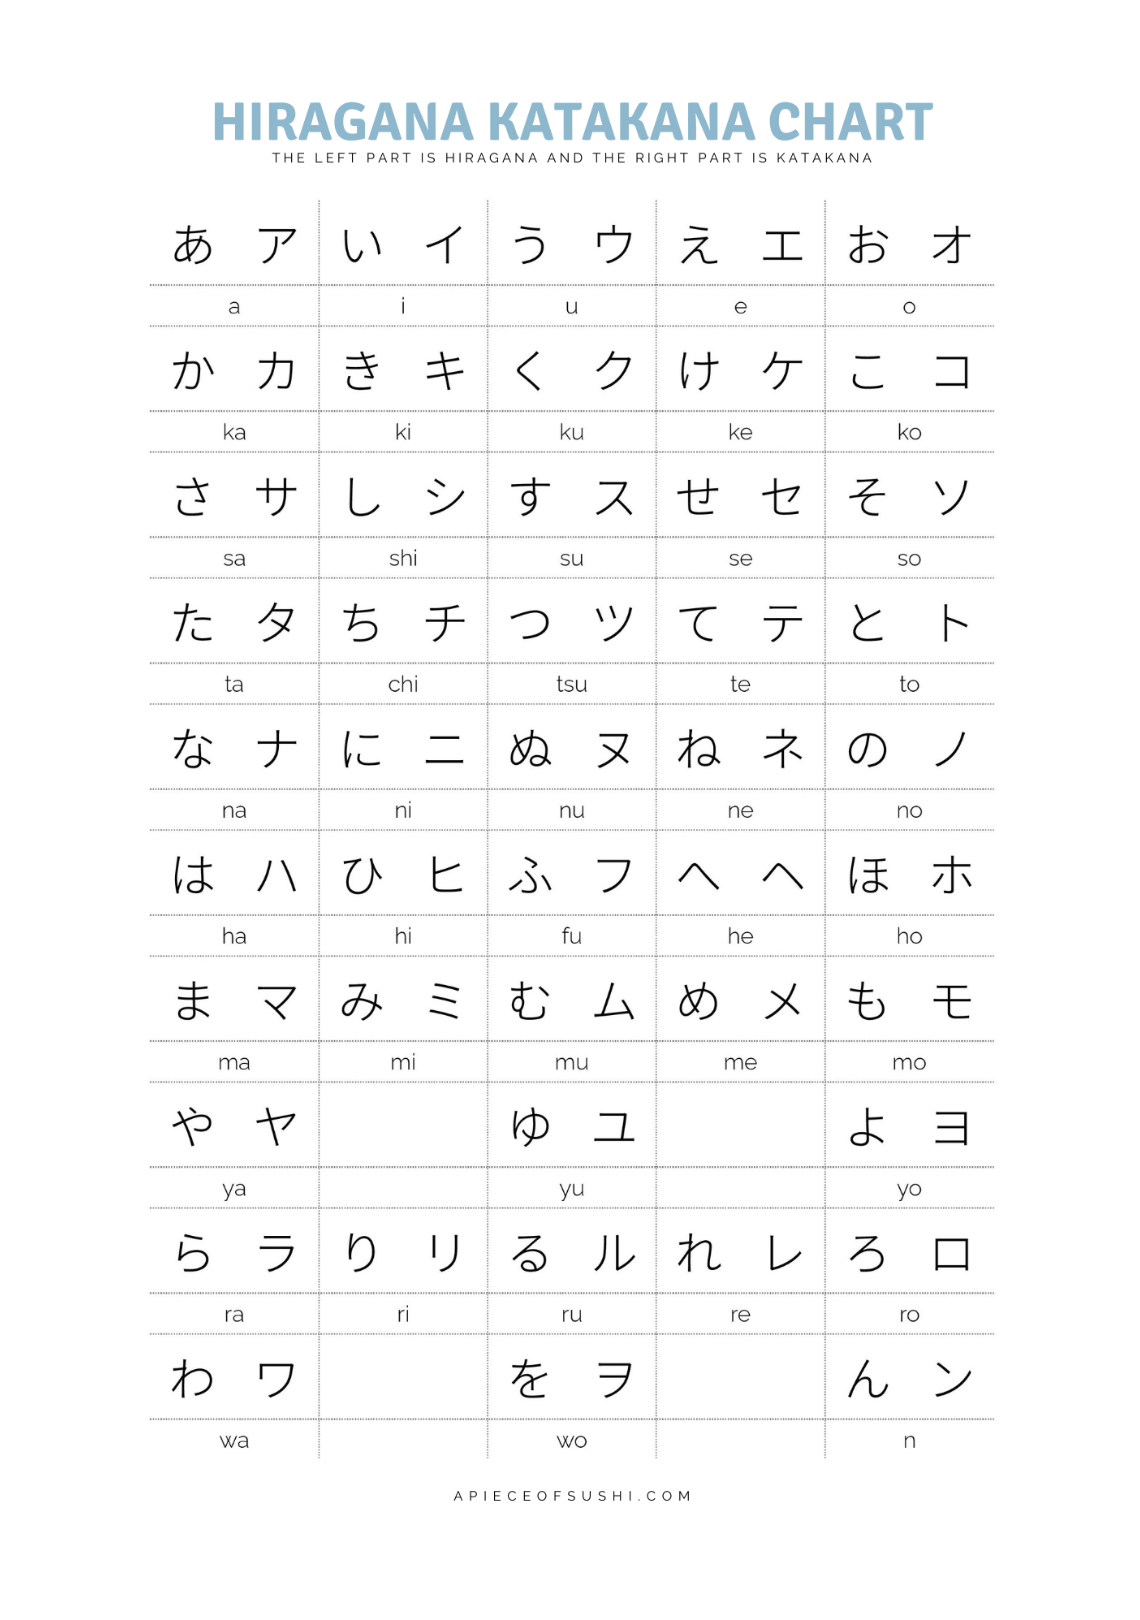
\includegraphics[scale=0.76]{Images/hiraganaKatakanaChart.png}

%%%%%%%%%%%%%%%%%%%%%%%%%%%%%%%%%%%%%%%%%%%%%%%%%%%%%%%%%%%%%%%%%%%%%%%%%%%%%%%%%%%%%%%%%%%%%%%%%%%
% END Hiragana/Katakana Chart
% START Particles
%%%%%%%%%%%%%%%%%%%%%%%%%%%%%%%%%%%%%%%%%%%%%%%%%%%%%%%%%%%%%%%%%%%%%%%%%%%%%%%%%%%%%%%%%%%%%%%%%%%

% Page Header
\section{Particles}

% Page Contents
\subsection{Topic/Subject (は)}
\begin{tabularx}{\textwidth}{X | X}
    Xは。(X-wa) & "X" is the topic of the sentence. \\
    わたしは。(wa-ta-shi-wa) & "I" is the topic of the sentence. \\
\end{tabularx}

\noindent\rule{\linewidth}{1pt}

\subsection{Declaratives (です)}
\begin{tabularx}{\textwidth}{X | X}
    Yです。(Y-de-su)& 〜is "Y". \\
    アメリカじんです (a-me-ri-ka-ji-n-de-su) & 〜is American (Person).\\
\end{tabularx}

\noindent\rule{\linewidth}{1pt}

\subsection{Possessives (の)}
\begin{tabularx}{\textwidth}{X | X}
    XのY。(X-no-Y) & "Y" belongs to "X". \\
    アメリカのじん。(a-me-ri-ka-no-ji-n) & An American (Person). \\
\end{tabularx}

\noindent\rule{\linewidth}{1pt}

\subsection{Telephone Numbers (の)}
\begin{tabularx}{\textwidth}{X | X}
    \#-\#。(\#-no-\#) & Hyphens in numbers are pronounced "no" \\
    ご-ぜろい。(go-no-ze-ro-i-chi) & 5-01 \\
\end{tabularx}

\noindent\rule{\linewidth}{1pt}

%%%%%%%%%%%%%%%%%%%%%%%%%%%%%%%%%%%%%%%%%%%%%%%%%%%%%%%%%%%%%%%%%%%%%%%%%%%%%%%%%%%%%%%%%%%%%%%%%%%
% END Particles
% START Week 1
%%%%%%%%%%%%%%%%%%%%%%%%%%%%%%%%%%%%%%%%%%%%%%%%%%%%%%%%%%%%%%%%%%%%%%%%%%%%%%%%%%%%%%%%%%%%%%%%%%%

% Page Header
\newpage
\section{Week 1}

% Page Contents
\subsection{あいさつ （挨拶）- Aisatsu}
\begin{tabularx}{\textwidth}{X | X}
    \toprule
    \textbf{Japanese (日本語)} & \textbf{English (英語)} \\
    \midrule
    おはよう。 & Good morning. \\
    おはようございます。 & Good morning (Polite). \\
    こんにちは。 & Good afternoon. \\
    こんばんは。 & Good evening. \\
    さようなら。 & Goodbye. \\
    おやすみ（なさい）。 & Goodnight. \\
    ありがとう。 & Thank you. \\
    ありがとうございます。 & Thank you (Polite). \\
    すみません。 & Excuse me. / I’m Sorry. \\
    いいえ。 & No. / Not at all. \\
    いってきます。 & I’ll go and come back. \\
    いってらっしゃい。 & Please go and come back. \\
    ただいま。 & I’m home. \\
    おかえり（なさい）。 & Welcome home. \\
    いただきます。 & Thank you for the meal (Before eating). \\
    ごちそうさまでした。 & Thank you for the meal (After eating). \\
    はじめまして。 & How do you do? \\
    ～です。 & I am... \\
    よろしくおねがいします。 & Nice to meet you. \\
    \bottomrule
\end{tabularx}

\subsection{じゅぎょうにべんりなひょうげん - Useful Classroom Expressions}
\begin{tabularx}{\textwidth}{X | X}
    \toprule
    \textbf{Japanese (日本語)} & \textbf{English (英語)} \\
    \midrule
    \textbf{TEACHER INSTRUCTIONS:} & \\
    きいてください。 & Please listen. / Please ask. \\
    いってください。 & Please speak. \\
    \_をかいてください。 & Please write \_. \\
    よんでください。 & Please read. \\
    リピートしてください。 & Please repeat (after me). \\
    しゅくだいください。 & Homework please. \\
    わかりましたか。 & Do you understand? \\
    \_ページをみてください。 & Please look at page... \\
    \hline
    \textbf{BOTH:} & \\
    もういちどいってください。& Please say it again. \\
    ちょっとまってください。& Please wait a moment. \\
    \hline
    \textbf{STUDENT QUESTIONS/REQUESTS:} & \\
    はい、わかりました。& Yes, I understand or Yes, I understood. \\
    いいえ、わかりません。& No, I don't understand or No, I don't know. \\
    ゆっくりいってください。& Please say it slowly. \\
    \_はなんですか。& What is this \_? \\
    えいごではなしてもいいですか。& May I speak in English? \\
    \_はにほんごでなんですか。& What is \_ in Japanese? \\
    \_はえいごでなんですか。& What is \_ in English? \\
    \bottomrule
\end{tabularx}

\subsection{すうじ（数字） - Suuji}
\begin{tabularx}{\textwidth}{X | X | X}
    \toprule
    \textbf{Japanese (日本語)} & \textbf{Kanji} & \textbf{English (英語)} \\
    \midrule
    ゼロ／れえ & 零 & 0 \\
    いち & 一 & 1 \\
    に & 二 & 2 \\
    さん & 三 & 3 \\
    よん／し／よ & 四 & 4 \\
    ご & 五 & 5 \\
    ろく & 六 & 6 \\
    なな／しち & 七 & 7 \\
    はち & 八 & 8 \\
    きゅう／く & 九 & 9 \\
    じゅう & 十 & 10 \\
    にじゅうに & 二十二 & 22 \\
    ひゃく & 百 & 100 \\
    にひゃくにじゅうに & 二百二十二 & 222 \\
    せん & 千 & 1000 \\
    にせんにひゃくにじゅうに & 二千二百二十二 & 2222 \\
    まん & 万 & 10000 \\
    にまんにせんにひゃくにじゅうに & 二万二千二百二十二 & 22222 \\
    \bottomrule
\end{tabularx}

\subsection{たんご（単語） - Vocabulary}
\begin{tabularx}{\textwidth}{X | X | X}
    \toprule
    \textbf{Japanese (日本語)} & \textbf{Kanji} & \textbf{English (英語)} \\
    \midrule
    \textbf{FROM SLIDES:} & & \\
    あさ & 朝 & Morning \\
    きせす & 季節 & Season \\
    すし & 寿司 & Sushi \\
    そと & 外 & Outside \\
    せかい & 世界 & The world \\
    あそこ & 彼処 & Over there \\
    あお & 青 & Blue \\
    こえ & 声 & Voice \\
    \hline
    \textbf{FROM WORKBOOK:} & & \\
    こい & NONE & Carp \\
    うえ & 上 & Above \\
    おか & 丘 & Hill \\
    あき & 秋 & Autumn \\
    いけ & 池 & Pond \\
    かく & 書く & Write \\
    あう & 会う & Meet \\
    いえ & 家 & House \\
    あい & 愛 & Love \\
    かお & 顔 & Face \\
    きく & 聞く & Listen \\
    とち & 土地 & Land \\
    かたて & 片手 & One Hand \\
    たすけ & 助け & Help \\
    ちかてつ & 地下鉄 & Subway \\
    かさ & 傘 & Umbrella \\
    とし & 年 & Age \\
    \bottomrule
\end{tabularx}

%%%%%%%%%%%%%%%%%%%%%%%%%%%%%%%%%%%%%%%%%%%%%%%%%%%%%%%%%%%%%%%%%%%%%%%%%%%%%%%%%%%%%%%%%%%%%%%%%%%
% END Week 1
% START Week 2
%%%%%%%%%%%%%%%%%%%%%%%%%%%%%%%%%%%%%%%%%%%%%%%%%%%%%%%%%%%%%%%%%%%%%%%%%%%%%%%%%%%%%%%%%%%%%%%%%%%

% Page Header
\newpage
\section{Week 2}

% Page Contents
\subsection{すうじ（数字歳）- Suuji (Age)}
〜さい。（〜歳。）
\vspace{5pt}

\begin{tabularx}{\textwidth}{X | X | X}
    \toprule
    \textbf{Japanese (日本語)} & \textbf{Kanji} & \textbf{English (英語)} \\
    \midrule
    \colorbox{yellow}{いっさい} & 一歳 & \colorbox{yellow}{1 years old} \\
    にさい & 二歳 & 2 years old \\
    さんさい & 三歳 & 3 years old \\
    よんさい & 四歳 & 4 years old \\
    ごさい & 五歳 & 5 years old \\
    ろくさい & 六歳 & 6 years old \\
    ななさい & 七歳 & 7 years old \\
    \colorbox{yellow}{はっさい} & 八歳 & \colorbox{yellow}{8 years old} \\
    きゅうさい & 九歳 & 9 years old \\
    じゅうさい & 十歳 & 10 years old \\
    にじゅうさい ・ \colorbox{yellow}{はたち} & 二十歳 & 20 years old \colorbox{yellow}{(Coming of age)} \\
\end{tabularx}
\noindent\rule{\linewidth}{1pt}

\subsection{すうじ（数字時）- Suuji (Time - Hours)}
〜じ。（〜時。）
Time in Japan often uses military time (2400 hour system) to refer to time.
\vspace{5pt}

\begin{tabularx}{\textwidth}{X | X | X}
    \toprule
    \textbf{Japanese (日本語)} & \textbf{Kanji} & \textbf{English (英語)} \\
    \midrule
    \colorbox{yellow}{れいじ} & 零時 & \colorbox{yellow}{Midnight - 12PM - 0000} \\
    いちじ & 一時 & 1 o'clock - 0100 \\
    にじ & 二時 & 2 o'clock - 0200 \\
    さんじ & 三時 & 3 o'clock - 0300 \\
    \colorbox{yellow}{よじ} & 四時 & \colorbox{yellow}{4 o'clock - 0400} \\
    ごじ & 五時 & 5 o'clock - 0500 \\
    ろくじ & 六時 & 6 o'clock - 0600 \\
    \colorbox{yellow}{しちじ} & 七時 & \colorbox{yellow}{7 o'clock - 0700} \\
    はちじ & 八時 & 8 o'clock - 0800 \\
    \colorbox{yellow}{くじ} & 九時 & \colorbox{yellow}{9 o'clock - 0900} \\
    じゅうじ & 十時 & 10 o'clock - 1000 \\
    じゅういちじ & 十一時 & 11 o'clock - 1100 \\
    じゅうにじ & 十二時 & 12 o'clock - 1200 \\
    じゅうさんじ & 十三時 & 13 o'clock - 1300 \\
    ごぜん〜 & 午前〜 & ~AM \\
    ごご〜 & 午後〜 & ~PM \\
    \bottomrule
\end{tabularx}

\newpage
\subsection{すうじ（数字分）- Suuji (Time - Minutes)}
〜ふん・ぷん・ぶん。（〜分。）

\vspace{5pt}

\begin{tabularx}{\textwidth}{X | X | X}
    \toprule
    \textbf{Japanese (日本語)} & \textbf{Kanji} & \textbf{English (英語)} \\
    \midrule
    \colorbox{yellow}{いっぷん} & 一分 & \colorbox{yellow}{1 minute} \\
    にふん & 二分 & 2 minutes \\
    \colorbox{yellow}{さんぷん} & 三分 & \colorbox{yellow}{3 minutes} \\
    \colorbox{yellow}{よんぷん} & 四分 & \colorbox{yellow}{4 minutes} \\
    ごふん & 五分 & 5 minutes \\
    \colorbox{yellow}{ろっぷん} & 六分 & \colorbox{yellow}{6 minutes} \\
    \colorbox{yellow}{ななふん} & 七分 & \colorbox{yellow}{7 minutes} \\
    \colorbox{yellow}{はっぷん・はちふん} & 八分 & \colorbox{yellow}{8 minutes} \\
    きゅうふん & 九分 & 9 minutes \\
    \colorbox{yellow}{じゅうぷん} & 十分 & \colorbox{yellow}{10 minutes} \\
    じゅういっぷん & 十一分 & 11 minutes \\
    じゅうにふん & 十二分 & 12 minutes \\
    \colorbox{yellow}{〜はん} & 〜半 & \colorbox{yellow}{30 minutes - Half past 〜o'clock} \\
    \bottomrule
\end{tabularx}

\subsection{たんご（単語）- Vocabulary (Monday Slides)}
\begin{tabularx}{\textwidth}{X | X | X}
    \toprule
    \textbf{Japanese (日本語)} & \textbf{Kanji} & \textbf{English (英語)} \\
    \midrule
    だいがく & 大学 & College / University \\
    こうこう & 高校 & Highschool \\
    がくせい & 学生 & Student \\
    だいがくせい & 大学生 & College Student \\
    りゅうがくせい & 留学生 & International Student \\
    せんせい & 先生 & Teacher / Professor \\
    〜ねんせい & 〜年生 & ...Year Student \\
    いちねんせい & 一年生 & First-Year Student \\
    せんこう & 専攻 & Major \\
    わたし & 私 & I \\
    ともだち & 友達 & Friend \\
    〜さん & NONE & Mr. / Ms. \\
    〜じん & 〜人 & ...People \\
    にほんじん & 日本人 & Japanese people \\
    いま & 今 & Now \\
    ごぜん & 午前 & AM \\
    ごご & 午後 & PM \\
    〜じ & 〜時 & o'clock \\
    いちじ & 一時 & One o'clock \\
    はん & 半 & Half \\
    にじはん & 二時半 & Half past two \\
    にほん & 日本 & Japan \\
    アメリカ & NONE & U.S.A \\
    〜ご & 〜語 & ...Language \\
    にほんご & 日本語 & Japanese language \\
    〜さい & 〜歳 & ...Years old \\
    でんわ & 電話 & Telephone \\
    〜ばん & 〜番 & Number...\\
    ばんごう & 番号 & Number \\
    なまえ & 名前 & Name \\
    なん/なに & 何 & What \\
    あのう。 & NONE & Um...\\
    はい。 & NONE & Yes \\
    そうです。 & NONE & That's right \\
    そうですか。 & NONE & I see. / Is that so? \\
    \bottomrule
\end{tabularx}

\subsection{たんご（単語）- Vocabulary (Wednesday Slides)}
\begin{tabularx}{\linewidth}{X | X | X}
    \toprule
    \textbf{Japanese (日本語)} & \textbf{Kanji} & \textbf{English (英語)} \\
    \midrule
    くに & 国 & Country \\
    イギリス & NONE & Britain \\
    アースとラリア & NONE & Australia \\
    かんこく & 韓国 & Korea \\
    カナダ & NONE & Canada \\
    ちゅうごく & 中国 & China \\
    インド & NONE & India \\
    エジプト & NONE & Egypt \\
    フィリピン & NONE & Philippines \\
    \hline
    せんこう & 専攻 & Major (Studies) \\
    アジアけんきゅう & アジア研究 & Asian Studies \\
    けいざい & 経済 & Economics \\
    こうがく & 工学 & Engineering \\
    こくさいかんけい & 国際関係 & International Relations \\
    コンピューター & NONE & Computer \\
    せいじ & 政治 & Politics \\
    せいぶつがく & 生物学 & Biology \\
    ビジネス & NONE & Business \\
    ぶんがく & 文学 & Literature \\
    れきし & 歴史 & History \\
    \hline
    しごと & 仕事 & Occupation \\
    いしゃ & 医者 & Doctor \\
    かいしゃいん & 会社員 & Office Worker \\
    かんごし & 看護師 & Nurse \\
    こうこうせい & 高校生 & Highschool Student \\
    しゅふ & 主婦 & Housewife \\
    しゅふ & 主夫 & Househusband \\
    だいがくいんせい & 大学院生 & Graduate Student \\
    べんごし & 弁護士 & Lawyer \\
    \hline
    かぞく & 家族 & Family \\
    おかあさん & お母さん & Mother \\
    おとうさん & お父さん & Father \\
    おねえさん & お姉さん & Older Sister \\
    おにいさん & お兄さん & Older Brother \\
    いもうと & 妹 & Younger Sister \\
    おとうと & 弟 & Younger Brother \\
    \bottomrule
\end{tabularx}
\newpage
\begin{tabularx}{\textwidth}{X | X | X}
    \toprule
    \textbf{Japanese (日本語)} & \textbf{Kanji} & \textbf{English (英語)} \\
    \midrule
    あき & 秋 & Autumn \\
    そと & 外 & Outside \\
    むすめ & 娘 & Daughter \\
    きつね & 狐 & Fox \\
    ふね & 船 & Boat, Ship \\
    やま & 山 & Mountain \\
    おゆ & お湯 & Hot Water \\
    あなた & 貴方 & You \\
    よむ & 読む & To read \\
    かく & 書く & To write \\
    もち & 餅 & Rice cake \\
    まつ & 待つ & To wait \\
    かみ & 紙 & Paper \\
    よやく & 予約 & Reservation \\
    \bottomrule
\end{tabularx}

\newpage
\subsection{たんご（単語）- Vocabulary (From Workbook)}
\begin{tabularx}{\linewidth}{X | X | X}
    \toprule
    \textbf{Japanese (日本語)} & \textbf{Kanji} & \textbf{English (英語)} \\
    \midrule
    ひふ & 皮膚 & Skin \\
    なにか & 何か & Something \\
    ほね & 骨 & Bone \\
    しね & 死ね & Die \\
    このは & 木の葉 & Leaf \\
    へた & 下手 & Clumsy \\
    ふね & 船 & Boat \\
    ほし & 星 & Star \\
    はな & 花 & Flower \\
    へそ & 臍 & Navel \\
    ぬの & 布 & Cloth \\
    ひにく & 皮肉 & Sarcasm \\
    まち & 町 & Town \\
    みせ & 店 & Store \\
    むね & 胸 & Chest \\
    ゆめ & 夢 & Dream \\
    もや & 靄 & Fog \\
    よむ & 読む & Read \\
    もち & 餅 & Rice Cake \\
    まつ & 待つ & Wait \\
    かみ & 紙 & Paper / Hair \\
    おゆ & お湯 & Hot Water \\
    むすめ & 娘 & Daughter \\
    よやく & 予約 & Reservation \\
    \bottomrule
\end{tabularx}

%%%%%%%%%%%%%%%%%%%%%%%%%%%%%%%%%%%%%%%%%%%%%%%%%%%%%%%%%%%%%%%%%%%%%%%%%%%%%%%%%%%%%%%%%%%%%%%%%%%
% END Week 2
% START Week 3
%%%%%%%%%%%%%%%%%%%%%%%%%%%%%%%%%%%%%%%%%%%%%%%%%%%%%%%%%%%%%%%%%%%%%%%%%%%%%%%%%%%%%%%%%%%%%%%%%%%

% Page Header
\newpage
\section{Week 3}

% Page Contents
\subsection{Placeholder}

%%%%%%%%%%%%%%%%%%%%%%%%%%%%%%%%%%%%%%%%%%%%%%%%%%%%%%%%%%%%%%%%%%%%%%%%%%%%%%%%%%%%%%%%%%%%%%%%%%%
% END Week 3
% START Week 4
%%%%%%%%%%%%%%%%%%%%%%%%%%%%%%%%%%%%%%%%%%%%%%%%%%%%%%%%%%%%%%%%%%%%%%%%%%%%%%%%%%%%%%%%%%%%%%%%%%%

% Page Header
\newpage
\section{Week 4}

% Page Contents
\subsection{Placeholder}

%%%%%%%%%%%%%%%%%%%%%%%%%%%%%%%%%%%%%%%%%%%%%%%%%%%%%%%%%%%%%%%%%%%%%%%%%%%%%%%%%%%%%%%%%%%%%%%%%%%
% END Week 4
% START Week 5
%%%%%%%%%%%%%%%%%%%%%%%%%%%%%%%%%%%%%%%%%%%%%%%%%%%%%%%%%%%%%%%%%%%%%%%%%%%%%%%%%%%%%%%%%%%%%%%%%%%

% Page Header
\newpage
\section{Week 5}

% Page Contents
\subsection{Placeholder}

%%%%%%%%%%%%%%%%%%%%%%%%%%%%%%%%%%%%%%%%%%%%%%%%%%%%%%%%%%%%%%%%%%%%%%%%%%%%%%%%%%%%%%%%%%%%%%%%%%%
% END Week 5
% START Week 6
%%%%%%%%%%%%%%%%%%%%%%%%%%%%%%%%%%%%%%%%%%%%%%%%%%%%%%%%%%%%%%%%%%%%%%%%%%%%%%%%%%%%%%%%%%%%%%%%%%%

% Page Header
\newpage
\section{Week 6}

% Page Contents
\subsection{Placeholder}

%%%%%%%%%%%%%%%%%%%%%%%%%%%%%%%%%%%%%%%%%%%%%%%%%%%%%%%%%%%%%%%%%%%%%%%%%%%%%%%%%%%%%%%%%%%%%%%%%%%
% END Week 6
% START Week 7
%%%%%%%%%%%%%%%%%%%%%%%%%%%%%%%%%%%%%%%%%%%%%%%%%%%%%%%%%%%%%%%%%%%%%%%%%%%%%%%%%%%%%%%%%%%%%%%%%%%

% Page Header
\newpage
\section{Week 7}

% Page Contents
\subsection{Placeholder}

%%%%%%%%%%%%%%%%%%%%%%%%%%%%%%%%%%%%%%%%%%%%%%%%%%%%%%%%%%%%%%%%%%%%%%%%%%%%%%%%%%%%%%%%%%%%%%%%%%%
% END Week 7
% START Week 8
%%%%%%%%%%%%%%%%%%%%%%%%%%%%%%%%%%%%%%%%%%%%%%%%%%%%%%%%%%%%%%%%%%%%%%%%%%%%%%%%%%%%%%%%%%%%%%%%%%%

% Page Header
\newpage
\section{Week 8}

% Page Contents
\subsection{Placeholder}

%%%%%%%%%%%%%%%%%%%%%%%%%%%%%%%%%%%%%%%%%%%%%%%%%%%%%%%%%%%%%%%%%%%%%%%%%%%%%%%%%%%%%%%%%%%%%%%%%%%
% END Week 8
% START Week 9
%%%%%%%%%%%%%%%%%%%%%%%%%%%%%%%%%%%%%%%%%%%%%%%%%%%%%%%%%%%%%%%%%%%%%%%%%%%%%%%%%%%%%%%%%%%%%%%%%%%

% Page Header
\newpage
\section{Week 9}

% Page Contents
\subsection{Placeholder}

%%%%%%%%%%%%%%%%%%%%%%%%%%%%%%%%%%%%%%%%%%%%%%%%%%%%%%%%%%%%%%%%%%%%%%%%%%%%%%%%%%%%%%%%%%%%%%%%%%%
% END Week 9
% START Week 10
%%%%%%%%%%%%%%%%%%%%%%%%%%%%%%%%%%%%%%%%%%%%%%%%%%%%%%%%%%%%%%%%%%%%%%%%%%%%%%%%%%%%%%%%%%%%%%%%%%%

% Page Header
\newpage
\section{Week 10}

% Page Contents
\subsection{Placeholder}

%%%%%%%%%%%%%%%%%%%%%%%%%%%%%%%%%%%%%%%%%%%%%%%%%%%%%%%%%%%%%%%%%%%%%%%%%%%%%%%%%%%%%%%%%%%%%%%%%%%
% END Week 10
% START Sources Cited
%%%%%%%%%%%%%%%%%%%%%%%%%%%%%%%%%%%%%%%%%%%%%%%%%%%%%%%%%%%%%%%%%%%%%%%%%%%%%%%%%%%%%%%%%%%%%%%%%%%

% Page Header
\newpage
\section{Sources Cited}

% Page Contents
\begin{itemize}
    \item Dr. Hammine, M. (2026).  \emph{Japanese 1001}. College of Arts, Humanities, \& Social Sciences, University of Denver.
    \item A Piece of Sushi. (2020). \emph{Hiragana + Katakana Chart}. \url{https://apieceofsushi.com/}.
    \item JapanDict. (2010-2026). \emph{JapanDict: Free online Japanese dictionary}. \url{https://www.japandict.com/}.
\end{itemize}

%%%%%%%%%%%%%%%%%%%%%%%%%%%%%%%%%%%%%%%%%%%%%%%%%%%%%%%%%%%%%%%%%%%%%%%%%%%%%%%%%%%%%%%%%%%%%%%%%%%
% END Sources Cited
%%%%%%%%%%%%%%%%%%%%%%%%%%%%%%%%%%%%%%%%%%%%%%%%%%%%%%%%%%%%%%%%%%%%%%%%%%%%%%%%%%%%%%%%%%%%%%%%%%%

\end{CJK}
\end{document}